\documentclass[a4j,11pt]{jsarticle}
\usepackage{semi}

\makeatletter % プリアンブルで定義開始

% 図番号を"<章節などの番号番号> - <図番号>" へ
\renewcommand{\thefigure}{\thesubsection-\arabic{figure}}
\renewcommand{\thetable}{\thesubsection-\arabic{table}}
% 章が進むごとに図番号をリセットする
\@addtoreset{figure}{subsection}
\@addtoreset{table}{section}

\makeatother % プリアンブルで定義終了

\renewcommand{\headfont}{\bfseries} %章タイトルなどを明朝体にする

\makeindex
\begin{document}
\definecolor{cellcolor}{rgb}{ 1, .90, .90}
\definecolor{rowcolor}{rgb}{.85, .85, 1}
\setcounter{tocdepth}{3}
\thispagestyle{empty}
\begin{center}

\huge
2020年度 卒業論文\\[60pt]
\HUGE
ケプストラム法を用いた\\
反射音除去の提案\\[65pt]
\huge
指導教員 須田 宇宙 准教授\\[40pt]
千葉工業大学 情報ネットワーク学科\\[10pt]
須田研究室\\[40pt]
1632033 \hspace{70pt} 岡田 秀\\[110pt]
\end{center}
\begin{flushright} 
\huge

\textcolor{white}{文字}

\textcolor{white}{文字}

提出日 2020年1月25日
\end{flushright}
\newpage
\thispagestyle{empty}
\large
% 目次
\tableofcontents

\newpage
%表目次
\listoftables
%図目次
\listoffigures

\begin{comment}

\end{comment}
\newpage

\section{緒言}

%背景+問題点
近年,災害が多発している中,町内放送などの非常放送が重要性を増している\cite{oka1}.屋外,デパートなどの屋内,トンネルの中など様々な場所で館内放送や非常放送の整備されている.しかし,スピーカから離れている地点で放送を聞くと建物などによる反射音により,内容を聞き取りづらいことが多い.ここで,信号処理によって反射音を除去できれば,放送内容を聞き取ることが可能となる.

火災が発生した場合,屋内のスピーカからの非常放送を屋内で受聴することになるが,反射や残響によって聞き取りづらいことが懸念される.
一方,建築音響の分野では,単発の信号音に対する反射音の時間遅れとその大きさを表す指標としてインパルス応答が用いられる.反射音を除去する方法として佐藤\cite{oka2}の研究では非常用放送の音声の先頭に信号音を付加させた.その信号音を基準とし,デジタルデバイスによってリアルタイムにインパルス応答を計算し,余分な反射音を除去する手法を提案した.しかし,クロススペクトル法の理論は正しかったが,実際の音声を用いて計算したところうまく動作しなかった.


%目的
本研究では,佐藤\cite{oka2}の研究の理論の部分を逆畳込みとケプストラム法を用いて非常放送を明瞭に聞き取ることを目的とする.

\subsection{行政放送などの公共放送における問題点}
行政放送や,公共放送などは津波や地震,火災といった人の命に関する放送することが多くある.そのような重要な放送は時と場所によっては内容が聞き取りづらい,または聞き取れない,ことがある.

一つ例を挙げるとすると2011年3月11日に発生した東日本大震災がある.被災地において,普段は行政無線などの広域拡散情報通信システムは,隣接するスピーカーからの音が重ならないよう,十分な時間間隔を開けて出力している.しかし,当時は津波の避難を迅速に行わなければいけないこと,自分自身も避難しなければいけないことなどがあり,十分な時間間隔を開けることができなく放送を行ってしまった.結果としてスピーカ同士の干渉であったり,建物などによる反射により内容を十分に聞き取ることができなかったという問題が発生した.


\newpage

\section{行政放送}
行政放送は市町村防災行政無線のことをいい,主に地方行政における無線の一種である.放送内容は大規模災害時の避難勧告や避難命令などの告知,火災発生の知らせといった非常時の放送を始め,朝・昼・夕方の時報を知らせる音楽.鐘・サイレン・チャイムや児童に帰宅を促す放送などがある.放送のほとんどは遠方にある野外スピーカからの声が重なって聞き取りにくくなるのを防ぐため,語間を大きく開け,ゆっくり話す,または,放送区域を時間差で切り替える時間差放送を行っているのが特徴である.

\newpage

\section{津波や地震や火事による自然災害}
津波は主に地震や火山活動による海底の地形の急変により,海洋に生じる大規模な波のことであり,自身による津波は海溝付近で発生することが多い.2011年に発生した東日本大震災の津波は観測史上最大級規模のの津波であり,震源地は仙台市の東方70km出会ったが,北海道から千葉県にかけて大津波が押し寄せている.

津波の伝搬する速度は水深と波の高さによって決まり,基本的には重力加速度に水深を乗じた値の平方根に等しくなっている.東日本大震災では震源地から岩手県重茂半島まで平均時速115kmで到達しており,津波の高さは同書で8.5mとなっている.しかい,津波が強すぎたためか観測データが送信されておらず,実際にはもっと高かった可能性もある.宮城県女川町では鉄筋コンクリート製のビルが基礎の部分から自演から抜けて横倒しになってしまっている.

津波の強さは,高さ1mでの破壊力があり,成人男性であっても死亡してしまう可能性がある.また,木造建築であれば全壊してしまう可能性がある.また,津波は陸から海へ引く,引波の際の力も強く,時折,湖岸で釣りをしていた釣り人が沖合に流されてしまうニュースもある.

地震が起きた際の津波の発生原理を示す.海底で地震が発生すると海底の地盤が動き,海側のプレートと陸側のプレートの隆起と沈降が起こる.プレートの隆起と沈降に合わせて上げ潮や引き潮が発生し,津波につながる.津波はお気から騎士につかづくほど波が高くなり,親水が深ければ深いほど速度が早くなる.

\newpage

\section{室内音響}
\subsection{残響音・反響}
室内などの閉空間内で発生した音は壁にあたって反射する.反射した音は別の壁による反射を繰り返し,次第に減少していく.このような多重の反射が作り出す現象を残響という.

\subsection{インパルス応答}
音源から単一の衝撃音を発したときの受音点での音の観測結果は例を図\ref{fig:impulse}に示す..直接音をインパルスと呼び,それに対する空間情報すべてをインパルス応答と呼ぶ\cite{oka3}.

\begin{figure}[h]
\begin{center}
 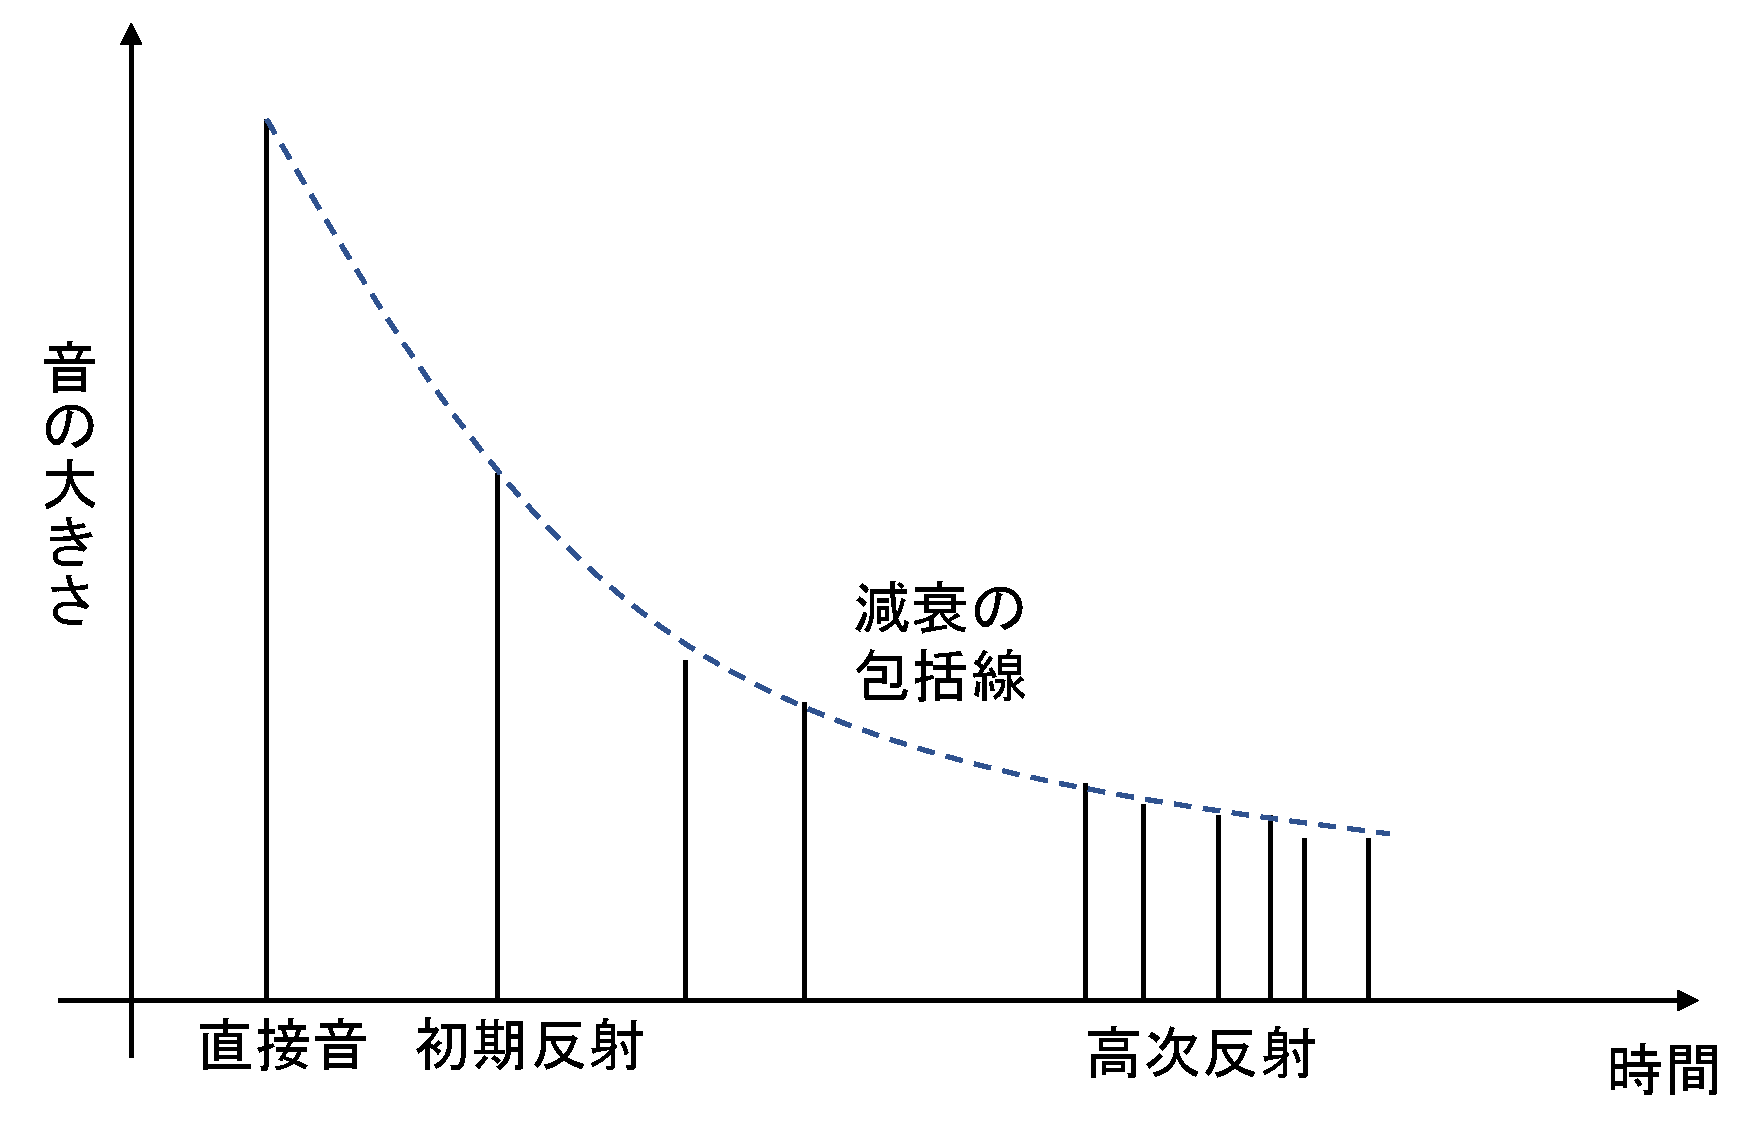
\includegraphics[clip,width=80mm,height=55mm]{ImpulseResponse.pdf}
\end{center}
 \caption{インパルス応答の例\cite{oka2}}
 \label{fig:impulse}
\end{figure}

\subsection{ノイズ}
\subsection{TSP信号}
\newpage

\section{信号処理}
信号処理とは,信号(光・音声・画像信号など)を数理手法で処理(分析・加工)する学問・技術の総称である.

アナログ信号処理とデジタル信号処理に分けられる.信号処理を支える基礎的な分野は信号理論とも呼ばれる.

基本的には,信号から信号に変換するものであり,信号とは別の形式の情報を得るもの(例えば、カテゴリ分けや関連づけ,推論的な情報を得る認識や理解など)は含まれない.圧縮も含まれないことが多い.但し,認識や理解,圧縮の前段階としての信号の変換は信号処理と呼ばれる.そのため,信号処理はそれらの技術に対して非常に重要であるとともに関連が強い.なお,また入力と出力が同じ種類(物理量)の信号である場合(例えば入力と出力ともに同じ音圧である場合)には,フィルタリングとも呼ばれる.

信号処理の例としては,ノイズの載った信号から元の信号を推定するノイズ除去や,時間的な先の値を推定する予測,時間周波数解析などを行う直交変換,信号の特徴を得る特徴抽出,特定の周波数成分のみを得るフィルタなどがある.

高速フーリエ変換,ウェーブレット変換,畳み込み等のアルゴリズムがあり,以前はそれぞれ専用のハードウェアで処理していたが,近年ではDSPや汎用のハードウェアでソフトウェアで処理したり,FPGAによる再構成可能コンピューティングによって処理する方法が開発されつつある.


\subsection{周波数特性.周波数領域}
\subsection{フーリエ変換}
\subsection{伝達関数}

\newpage

\section{反射音除去の一提案}
\subsection{先行研究による手法}
非常放送には反射音が建物などにより付加してしまい内容を聞き取りづらいといったことが問題点として挙げられている.その反射音を除去するために佐藤はクロススペクトル方を用いて反射音の除去に取り組んだ.

手法としては元波形の前におらかじめ信号音を付加させておく.それをもとに反射度合いを推定するため,インパルス応答を求める.反射音の付加された音声をインパルス応答で割ることで反射音が除去できる.

計算内容としては元波形を$S(t)$,反射音の含まれた音声を$R(t)$とすると,
はじめに両波形をフーリエ変換することにより周波数成分を求める.

\begin{equation}
  S(f) = \mathcal{F}[S(t)]
\end{equation}

\begin{equation}
  R(f) = \mathcal{F}[R(t)]
\end{equation}
 
元波形の周波数成分を二乗する(\ref{power})ことでパワースペクトル$P(f)$,元波形の周波数成分と反射音の含んだ波形の周波数成分の積(\ref{cross})によりクロススペクトル$C(f)$を求めることができる.
\begin{equation}
	\label{power}
  P(f) = [S(f)]^2
\end{equation}

\begin{equation}
	\label{cross}
  C(f) = [S(f)]・[R(f)]
\end{equation}

クロススペクトルをパワースペクトルで除算すること(\ref{transfer})により伝達関数$H(f)$を求めることができ,伝達関数を逆フーリエ変換すること(\ref{IR})によりインパルス応答$IR(t)$を求めることができる.
\begin{equation}
	\label{transfer}
  H(f) = \frac{C(f)}{P(f)}
\end{equation}

\begin{equation}
	\label{IR}
  IR(t) = \mathcal{F}^{-1}[H(f)]
\end{equation}

求めたインパルス応答を用いて,反射音の付加している音声の周波数成分をインパルス応答で除算すること(\ref{norefcomp})により反射音の除去された音声の周波数成分$N(f)$を求めることができる.またそれを逆フーリエ変換すること(\ref{noref})により反射音の除去された音声$N(t)$を取り出すことができる.

\begin{equation}
	\label{norefcomp}
  N(f) = \frac{R(f)}{IR(t)}
\end{equation}

\begin{equation}
	\label{noref}
  N(t) = \mathcal{F}^{-1}[N(f)]
\end{equation}

\begin{equation}
  %N(t)\fallingdotseq S(t)
\end{equation}

\newpage

\subsection{提案手法}
\subsection{ケプストラム法}
\subsection{逆畳み込み}

\newpage

\section{実験と検証}
\subsection{調査目的と調査方法}
\subsection{回答の集計と効果の検証}
\subsection{考察}

\newpage
\section{結言}

\newpage
\section*{謝辞}
\addcontentsline{toc}{section}{謝辞}
ここに研究の謝辞.主にご協力いただいた方など.

\newpage
\bibliographystyle{jplain}
\addcontentsline{toc}{section}{参考文献}
\begin{thebibliography}{99}

\bibitem{oka1}国土技術センター,"自然災害の多い国",http://www.jice.or.jp/knowledge/japan/commentary09
\bibitem{oka2}佐藤 由希子,"インパルス応答を用いた反射音除去のための一提案", 千葉工業大学卒業論文, 2014
\bibitem{oka3}小泉 宣夫,"基礎音響・オーディオ学",コロナ社 2005 36-38頁

\end{thebibliography}

\newpage
\section*{付録}
\addcontentsline{toc}{section}{付録}

\end{document}
